\documentclass{report}
\usepackage{graphicx}
\usepackage{float}
\usepackage{fullpage}
\usepackage{array}

\setlength{\extrarowheight}{4pt}

\graphicspath{{./images/}}

\floatstyle{boxed}
\restylefloat{figure}
<<<<<<< HEAD
\title{Green, Aware, and Responsive Total Home}
\author{Ben Ridder, Casey Banner, Zack MacLennan}
=======
%\title{Green, Automated, R Home T}
%\author{Ben Ridder, Casey Banner, Zack Mac}
>>>>>>> 525215603587eab63b2ccfa97bec51be06193ed1

\begin{document}
\begin{titlepage}
\begin{center}
\vfill
\hfill
\\[2cm]
\textsc{\LARGE University Of Waterloo}
\\[1cm]
\textsc{\LARGE ECE 355}
\\[2cm]

\hrule
\hfill
\\[0.5cm]
\textsc{\huge Software Requirements Specification}
\\[0.5cm]
\textsc{\huge GARTH}
\\[0.5cm]
\textsc{\huge Green, Aware, and Responsive Total Home}
\\[0.5cm]
\hrule
\hfill
\\[1cm]
\textsc{\LARGE Group 16} \\[0.4cm]

\begin{minipage}{0.4\textwidth}
\begin{flushleft} \large
Ben Ridder \\
Casey Banner \\
Zack MacLennan
\end{flushleft}
\end{minipage}
\begin{minipage}{0.4\textwidth}
\begin{flushright} \large
brridder \\
20299452 \\
20305946 
\end{flushright}
\end{minipage}


\vfill

{\large \today}
\end{center}
\end{titlepage}

%\maketitle
\tableofcontents
\listoffigures

\chapter{Introduction}
\section{Executive Summary}

\section{Purpose}

\section{Objectives}

\section{Scope}

\section{Terminology and Definitions}

%\section{Standards and References}

\chapter{Functional Requirements}

\section{High-level functionality}
The high level functionality of this system can be broken down into several
major sections. Sensors play a major role in interfacing the real world with
the several other sections of the controller. Physical security, both inside
and outside of the home is important. This goes hand in hand with family
security once family members have left the premises of the household. Finally,
green energy management can be easily integrated with the other systems to
ensure prudent usage of resources. 

\subsection{Sensors}
% TODO :: proof read this. It may not all make sense

% TODO :: elaborate HVAC or put it in the glossary
The most crucial part of the system that ties all of the other parts together
is the sensor network. They are the interface between the real world and the
controllers. They detect if the house has been intruded upon by outsiders
through sensors on the windows and doors. They can alert the family if somebody
left the stove top on. Living patterns can be established and monitored to warn
of health problems or to control the HVAC so that energy is not wasted when
nobody is home or they are all asleep. Cameras, motion detectors, hall effect
sensors, and other miscellaneous sensors comprise the majority of this network.

Cameras play multiple roles in the sensor network. Cameras positioned outside
the home will monitor activity throughout the day, with particular attention paid
to the entrances to the home. If an intruder approaches the home and tries to
break in, cameras will have filmed the incident in hopes to be able to identify
the trespeasser regardless of whether or not the break-in attempt was successful.
Footage will be stored in a database and then deleted after a certain period of
time.

Motion detectors provide the security system with the means to trigger alerts 
when motion is detected in certain areas of the home while the system is armed.
A network of motion detector sensors will be positioned in the hallways of the
home, with particular attention to entries to the home. Motion detectors
outside the house will be able to control the lighting system such that people
approaching the home can be illuminated and easily identified.

Temperature sensors and hall effect sensors are two other major components.
Temperature sensors can be used by both physical security, to ensure that the
oven has not been on for an extended period of time without user interaction as
well as for green energy management to control the overall temperature of the
house or each room. Hall effect sensors can be used with temperature sensors to
detect if windows or doors have been left open when they should be closed in
order to prevent wasting energy. These sensors can also be used to detect
intruders attempting to break in through windows or doors.

\subsection{Family Safety}

In addition to necessary home security functionality, the system will
incorporate methods to provide safety to members of the users' family. Child
safety is a particular concern that will be addressed by this portion of the
home security system. Sensors will be implemented on cabinets as well as
certain areas of the home that may contain hazardous materials that could be
harmful to children. Contact sensors will be present on medicine cabinets,
closets with cleaning materials, and knife drawers to alert the user that these
areas of the home have been accessed. Unlike the home security system
included in GARTH, these sensors are always active and do not need to be
armed to function properly. 

Child bedroom safety is also important, and can be part of a system catered 
towards families with infants who still sleep in cribs. Sensors in the child's room 
will be able to detect movement throughout the night to alert the parents of any 
disturbances. This system can be armed by the parents after putting their child
to sleep for the night via a console in the bedroom.

\subsection{Home Security System}

The home security system is one of main aspects of the GARTH system as a
whole. Like many modern home security systems it has two main states; armed
and disarmed. Users can arm the system via the consoles near the exits to the
home, using either a keypad code or an NFC device. Once armed, the security
system is in a ready state that will react to sensor inputs such as the window
sensors, hallway motion detectors, and other unauthorized home entry sensors.
If these sensors detect unexpected activity while armed, a critical alarm is sounded.
Other home security subsystems include basement flood detection, carbon 
monoxide detection, and warnings if the oven and/or stove have been left on
for extended periods of time.

\subsection{Green Energy Management}

Another aspect of the GARTH system is its green energy monitoring system. The
system includes a few ways to provide the user with green energy savings by
monitoring wasteful activity in the home. For example, sensors on the fridge and 
the freezer will be ready to detect if their doors have been left open for a long period
of time and will alert the user. One of the main ways that GARTH accomplishes
green energy management of the home is by monitoring and controlling thermostat 
usage. If the homeowners leave the thermostat on when nobody is home, the
system will alert the user to turn the thermostat off remotely. Also, GARTH includes
a smart control of the thermostat overnight such that the system runs in a high-efficiency
mode during the night when heat in the home is not as important.

\section{Scenarios}

\subsection*{Arming the System - NFC Device}

The resident is leaving the home and wishes to arm the security system. The
resident can do so by approaching the security console and tapping their NFC
device against the console. The resident must hold their NFC
device near the console until the device is read and identified by the system
as belonging to the resident of the home. Once this is confirmed, the user may
leave the home while the system initiates the arm countdown. Once the system
completes the countdown, the system has been successfully armed.

\subsection*{Disarming the System - NFC Device}

The procedure for disarming the system using an NFC device is very similar to
the arming procedure. The resident enters the home at which point the disarm
countdown begins. The resident holds his NFC device up to the console to disarm
the system. The NFC device is identified and the security system is disarmed
and the countdown is interrupted.

\subsection*{Arming the System - Keypad}

The resident wishes to arm the security system, but is not in possession of an
NFC device.  The resident can arm the system by entering a valid security code.
Once the code has been entered, it is validated by the system. The system
initiates the arm countdown, and the resident may now leave the home. The arm
countdown completes and the system is now armed.

\subsection*{Disarming the System - Keypad}

The procedure for disarming the system using the keypad is very similar to the
arming procedure. The resident enters the home at which point the disarm
countdown begins. The resident enters a valid security code into the console
using the keypad to disarm the system.  The NFC device is identified and the
security system is disarmed and the countdown is interrupted.

\subsection*{System Armed - Door Unlocked}

The resident arms the system, and leaves the house without locking the door.
A very brief countdown begins waiting for the door to lock. The countdown
ends and a loud audible beeping is emitted from a speaker near the door. The
resident returns and locks the door, at which point the beeping ceases.
Similarly if the resident leaves and does not notice that he has forgotten to
lock the door, the beeping ceases after a timeout and informs the resident with
an SMS.

\subsection*{Window Intrusion}
%TODO what happens during the alarm state?

The security system is in the armed state. An intruder attempts to open a
window from outside the home. The system receives a signal from the window's
sensor that notifies the system that a window has been opened. The system
enters its alarm state.

\subsection*{Door Intrusion}
%TODO what happens during the alarm state?

The security system is in the armed state. An intruder picks the lock on the
front door and opens it.  The system begins the alarm countdown alongside
audible beeping once the intruder opens the door.  The intruder leaves the
premises while the countdown continues. The countdown reaches zero and the
system enters the alarm state.

\subsection*{Fridge Left Open}

The resident opens the fridge door for a drink, and does not close it fully.
Unaware, the resident leaves the kitchen and sits down in the living room.
Meanwhile, a countdown has begun while the fridge door remains open. The
countdown finishes and a notification is sent to the resident via SMS. The
kitchen speaker broadcasts an audible message stating that the fridge door has
been left open. The user enters the kitchen and closes the fridge door,
resetting the system. 

\subsection*{Childproof Cabinets}

A child in the home has accessed a cabinet that contains hazardous or dangerous
materials. The contact sensor installed on the cabinet door triggers a
countdown. When the countdown reaches zero, and audible alarm is produced and
an SMS is sent to the resident of the home to notify them of the event.

Separately, an adult resident of the home accesses the same cabinet. The
contact sensor on the cabinet door triggers the countdown. The resident pushes
a hidden actuator located on the inside of the cabinet to halt the countdown.
The resident closes the cabinet door when he / she is finished and the sensor
notifies the process to go back to its normal wait state.

\subsection*{Child Bedroom Safety}
% TODO how does the resident arm the child safety system? With their phone?
% Console in the bedroom? 

The resident of the home has placed his child in the crib for the night. When
the resident leaves the bedroom, he arms the child bedroom safety system and
closes the door. During the middle of the night, the child climbs out the crib
and falls to the floor. Motion sensors installed in the room detect this
unexpected activity and sound an alarm in the parents' bedroom to notify them
of the event.

\subsection*{Carbon Monoxide Detection}

The furnace malfunctions and carbon monoxide gas begins leaking into the
basement. The basement's carbon monoxide detector senses that CO levels are
rising and alerts resident via SMS. Carbon monoxide continues to leak and the
allowable CO level has been reached. The carbon monoxide detector goes into its
alarm state, notifying the resident via SMS and sounding an audible alarm
throughout the house.

\subsection*{Flood Detection}
%TODO define alarm states (minor, intermediate, major?)

The basement's sump pump fails and groundwater begins to seep into the
basement.  Flood detectors installed in the system detect that water has risen
above the acceptable level. The resident is notified via SMS that the basement
is flooded, and a minor alarm is sounded throughout the home to alert the
residents of the flood.

\subsection*{Thermostat Left On}
%TODO define home inactivity

The residents of the home have the thermostat set to hold at 73 degrees
Fahrenheit.  The residents leave for vacation, but forget to turn the
thermostat off. After 24 hours of home inactivity, the system sends an SMS to
the resident to let them know that the thermostat has been set while nobody has
been home for 24 hours. The resident replies to the SMS which then turns the
thermostat off.

\section{Use case model}

\newlength{\originalParindent}
\setlength{\originalParindent}{\parindent}
\newlength{\originalParskip}
\setlength{\originalParskip}{\parskip}
\parindent 0pt
\parskip 10pt

\begin{tabular}{| l | p{12cm} |}
\hline
Use case name & \texttt{NFCDisarmSystem} \\ \hline
Participating Actors & Initiated by \texttt{Resident} \\ \hline
Flow of Events & 

\begin{enumerate}
 \item The \texttt{Resident} enters the home while in possession of an NFC 
        device.
 \item The system begins the disarm countdown.
 \item The \texttt{Resident} approaches the console and tapping the NFC device
       against the console.
 \item The data on the NFC device is read and validated by the system.
 \item The system enters the disarmed state and the disarm countdown is halted.
\end{enumerate}

\\ \hline

Entry Condition & The system is in the armed state and the Resident enters the
home in possession an NFC device. \\ \hline

Exit Condition & The system is disarmed. \\ \hline
Quality requirements & TODO \\ \hline

\hline
\end{tabular}

\begin{tabular}{| l | p{12cm} |}
\hline
Use case name & \texttt{KeyPadDisarmSystem} \\ \hline
Participating Actors & Initiated by \texttt{Resident} \\ \hline
Flow of Events & 

\begin{enumerate}
 \item The \texttt{Resident} enters the home.
 \item The system begins the disarm countdown.
 \item The \texttt{Resident} approaches the console and enters their code using
       the keypad on the console.
 \item The entered code is validated by the system.
 \item The system enters the disarmed state and the disarm countdown is halted.
\end{enumerate}

\\ \hline

Entry Condition & The system is in the armed state and the Resident
enters the home. \\ \hline

Exit Condition & The system is disarmed. \\ \hline
Quality requirements & TODO \\ \hline

\hline
\end{tabular}

\begin{tabular}{| l | p{12cm} |}
\hline
Use case name & \texttt{NFCArmSystem} \\ \hline
Participating Actors & Initiated by \texttt{Resident} \\ \hline
Flow of Events & 

\begin{enumerate}
 \item The \texttt{Resident} approaches the console and taps their NFC device
       against the console.
 \item The data on the NFC device is read and validated by the system.
 \item The system begins the arm countdown.
 \item The \texttt{Resident} leaves the home.
 \item The system arm countdown completes and the system enters the armed state.
\end{enumerate}

\\ \hline

Entry Condition & The system is in the disarmed state and the \texttt{Resident}
wishes to arm it using an NFC device. \\ \hline

Exit Condition & The system is armed. \\ \hline
Quality requirements & TODO \\ \hline

\hline
\end{tabular}

\begin{tabular}{| l | p{12cm} |}
\hline
Use case name & \texttt{KeyPadArmSystem} \\ \hline
Participating Actors & Initiated by \texttt{Resident} \\ \hline
Flow of Events & 

\begin{enumerate}
 \item The \texttt{Resident} approaches the console and enters their code.
 \item The entered code is validated by the system.
 \item The system begins the arm countdown.
 \item The \texttt{Resident} leaves the home.
 \item The system arm countdown completes and the system enters the armed state.
\end{enumerate}

\\ \hline

Entry Condition & The system is in the disarmed state and the \texttt{Resident}
    wishes to arm it using the keypad. \\ \hline
Exit Condition & The system is armed. \\ \hline
Quality requirements & TODO \\ \hline

\hline
\end{tabular}

\begin{tabular}{| l | p{12cm} |}
\hline
Use case name & \texttt{WindowIntrusionAlarm} \\ \hline
Participating Actors & Initiated by any actor. \\ \hline
Flow of Events & 

\begin{enumerate}
 \item A window is opened.
 \item The system receives the signal that the window has been opened.
 \item The system enters the alarm state.
\end{enumerate}

\\ \hline

Entry Condition & The system is in the armed state and a window is opened. \\ 
\hline
Exit Condition & The system alarm is triggered. \\ \hline
Quality requirements & TODO \\ \hline

\hline
\end{tabular}

\begin{tabular}{| l | p{12cm} |}
\hline
Use case name & \texttt{DoorIntrusionAlarm} \\ \hline
Participating Actors & Initiated by any actor. \\ \hline
Flow of Events & 

\begin{enumerate}
 \item A door is opened.
 \item The system begins the alarm countdown.
 \item The initiating actor does not disarm the system.
 \item The alarm countdown reaches zero.
 \item The system enters the alarm state.
\end{enumerate}

\\ \hline

Entry Condition & The system is in the armed state and a door is opened. \\ \hline
Exit Condition & The system alarm is triggered. \\ \hline
Quality requirements & TODO \\ \hline

\hline
\end{tabular}

\begin{tabular}{| l | p{12cm} |}
\hline
Use case name & \texttt{FridgeOpenNotification} \\ \hline
Participating Actors & Initiated by any actor. \\ \hline
Flow of Events & 

\begin{enumerate}
 \item The initiating actor opens the fridge door.
 \item The system begins a countdown.
 \item The countdown completes without the fridge door being closed.
 \item A notification is broadcast via SMS and the kitchen speaker, depending on configuration.
\end{enumerate}

\\ \hline

Entry Condition & Fridge door is opened. \\ \hline
Exit Condition & A ``fridge has been left open'' notification is broadcast. \\ \hline
Quality requirements & TODO \\ \hline

\hline
\end{tabular}

\begin{tabular}{| l | p{12cm} |}
\hline
Use case name & \texttt{CabinetAlarm} \\ \hline
Participating Actors & Initiated by any actor. \texttt{Resident} is a participant. \\ \hline
Flow of Events & 

\begin{enumerate}
 \item A secure cabinet is opened by the initiating actor.
 \item The contact sensor within the cabinet is tripped and a countdown begins.
 \item The countdown timer reaches zero.
 \item An audible alarm is produced by the system and an SMS is sent to the
       \texttt{Resident} notifying them of the intrusion.
\end{enumerate}

\\ \hline

Entry Condition & A secure cabinet is opened. \\ \hline
Exit Condition & An audible alarm is produced and an SMS alert is sent to
                 the \texttt{Resident} \\ \hline
Quality requirements & TODO \\ \hline

\hline
\end{tabular}

\begin{tabular}{| l | p{12cm} |}
\hline
Use case name & \texttt{CabinetAccess} \\ \hline
Participating Actors & Initiated by \texttt{Resident}. \\ \hline
Flow of Events & 

\begin{enumerate}
 \item A secure cabinet is opened by the \texttt{Resident}.
 \item The contact sensor within the cabinet is tripped and a countdown begins.
 \item The \texttt{Resident} pushes a hidden actuator within the cabinet.
 \item The countdown timer is stopped.
 \item The \texttt{Resident} closes the cabinet after they are finished.
\end{enumerate}

\\ \hline

Entry Condition & A secure cabinet is opened. \\ \hline
Exit Condition & The secure cabinet is closed. \\ \hline
Quality requirements & TODO \\ \hline

\hline
\end{tabular}

\begin{tabular}{| l | p{12cm} |}
\hline
Use case name & \texttt{ChildMotionDetected} \\ \hline
Participating Actors & Initiated by \texttt{Child}. \texttt{Resident} participates. \\ \hline
Flow of Events & 

\begin{enumerate}
 \item The child moves within the room.
 \item Motion sensors detect the movement and compare it to acceptable ranges.
 \item If the motion is out of the acceptable range, the child motion
       detector enters the alarm state and an alarm is sounded in the
       \texttt{Resident}'s bedroom.
\end{enumerate}

\\ \hline

Entry Condition & The child motion detector is in the armed state and the child moves
                  out of the acceptable range. \\ \hline
Exit Condition & Alarm is sounded in the \texttt{Resident}'s bedroom. \\ \hline
Quality requirements & TODO \\ \hline

\hline
\end{tabular}

\begin{tabular}{| l | p{12cm} |}
\hline
Use case name & \texttt{CarbonMonoxideDetected} \\ \hline
Participating Actors & \texttt{Resident} participates. \\ \hline
Flow of Events & 

\begin{enumerate}
 \item Sensors installed in the house detect that carbon monoxide (CO) levels have
       risen above acceptable values.
 \item SMS messages are sent to \texttt{Resident} alerting them of rising CO levels.
 \item If the CO levels continue to rise above a predefined level, the carbon monoxide
       detector goes into its alarm state. SMS message are again sent to \texttt{Resident}
       and an audible alarm is sounded throughout the house.
\end{enumerate}

\\ \hline

Entry Condition & Carbon monoxide levels in the home rise above an acceptable level. \\ \hline
Exit Condition & SMS messages are sent to \texttt{Resident} and an audible
                 alarm is sounded. \\ \hline
Quality requirements & TODO \\ \hline

\hline
\end{tabular}

\begin{tabular}{| l | p{12cm} |}
\hline
Use case name & \texttt{FloodDetected} \\ \hline
Participating Actors & \texttt{Resident} participates. \\ \hline
Flow of Events & 

\begin{enumerate}
 \item Flood detectors installed in the basement detect rising water levels.
 \item \texttt{Resident} is notified of the flood via SMS message and a minor alarm
       is sounded throughout the home.
\end{enumerate}

\\ \hline

Entry Condition & Rising water levels are detected by flood sensors. \\ \hline
Exit Condition & \texttt{Resident} is sent an SMS message and a minor alarm
                 is sounded throughout the home. \\ \hline
Quality requirements & TODO \\ \hline

\hline
\end{tabular}

\begin{tabular}{| l | p{12cm} |}
\hline
Use case name & \texttt{ThermostatReminder} \\ \hline
Participating Actors & \texttt{Resident} participates. \\ \hline
Flow of Events & 

\begin{enumerate}
 \item The \texttt{Resident} sets the house thermostat to hold a particular temperature.
 \item The \texttt{Resident} arms the system. A thermostat hold timer begins counting.
       this timer will be reset if the system is disarmed.
 \item Once the timer reaches 24 hours, the system sends an SMS message to the \texttt{Resident}
       to notify them that the thermostat has been in the hold state for 24 hours.
 \item The \texttt{Resident} replies to the SMS message.
 \item The system receives the SMS message from \texttt{Resident} and takes the thermostat
       out of the hold temperature state, resuming the normal thermostat schedule.
\end{enumerate}

\\ \hline

Entry Condition & The \texttt{Resident} sets the house thermostat to hold a particular
                  temperature. \\ \hline
Exit Condition &   \\ \hline
Quality requirements & TODO \\ \hline

\hline
\end{tabular}


% Reset floats back to normal and restore original parindent and parskip
\setlength{\parindent}{\originalParindent}
\setlength{\parskip}{\originalParskip}

\section{Object model}

\floatstyle{plain}
\restylefloat{figure}
\begin{figure}[hp]
    \centering
        \caption{Controller Class Diagram}
        \scriptsize
        \setlength{\unitlength}{2.0em}
        \includegraphics{classes1.mps}
        \normalsize
    \label{fig:controller_class_diagram}
\end{figure}
\floatstyle{boxed}
\restylefloat{figure}

\section{Dynamic model}


\section{Interfaces}
There are two interfaces between the components. The sensors need a way to
communicate to the controller their current data and the controller needs to
communicate to the actuators. Data from the controller needs to be sent to a
central server, which is then accessible through other user interfaces. The following
interfaces will help fulfill these requirements.

There are several interfaces between the system and the users to inform and
alert them of any issues. SMS text messages can be sent to the home owners if
any alarms have been tripped. If the owner does not acknowledge the issue, then
it is escalated to the security company for them judge the problem and if required,
call the local emergency services. Two user interfaces are provided to display
data and set system states. The first is a mobile application and the second is
a web interface. These user interfaces are described in more detail in
Chapter~\ref{ch:user-interfaces}

\subsection{Physical Hardware and Controller}
%TODO :: rename section?
The hardware, such as sensors and actuators, communicate wirelessly through
bluetooth to the controller. Two way communication is required as the hardware
needs to be able to register with the controller. The controller will also be
able to poll each sensor on a regular schedule to ensure that they are
operational and functioning properly. Examples of these sensors include
temperature, motion, and hall effect sensors. Some sensors need to report their
status when an event occurs so the controller interface needs to be able to
handle tight polling with interrupts to correctly collect all data.

\subsection{Server}
The server acts as the man in the middle interface between the controller and
the graphical user interfaces. The controller sends data, as appropriate, to
the server on a regular basis. This includes valuable information such as
a timestamped log file that records system events as well as periodic system
behaviour such as house temperature and arm states. The server stores the data in a 
database. The user accesses the data and can send state updates through an API 
exposed by the web server. This interface would allow an admin user to view the
logs, as well as see information about the system such as the system's firmware 
version. Network information such as the MAC addresses, and IP addresses of 
networked devices would also be available to the admin user from this interface.

\subsection{System Alerts to Homeowner}
Besides the physical interfaces such as the hardware controller and user
interfaces, the system alerts need to be interfaced with the user. The
interaction between the system and the user needs to follow an escalation
system to ensure that alarms are responded to appropriately and quickly.

Figure~\ref{fig:system_to_user_chart} shows the required flow of the escalation
path. When an alarm is triggered, the system should first send an SMS message
to the homeowner and wait a minimum period of time for a response via another
SMS reply or a phone call. If the homeowner responses, then end the alarm
state. Otherwise, inform the security company of the issue. The security
company then calls the homeowner. If the homeowner picks up the call, then end
the alarm state. Otherwise, the company needs to make an informed decision
based on the severity of the alarm to either send one of their own employees
or to call the local emergancy services. End the alarm state at this point.

\begin{figure}[hp]
    \centering
        \caption{System Alerts to Homeowner Escalation Flow Chart}
        \scriptsize
        \setlength{\unitlength}{2.0em}
        \begin{picture}(15.000000,20.000000)(-1.000000,-20.000000)
% picture environment flowchart generated by flow 0.99f
\put(2.0000,-1.0000){\oval(4.0000,2.0000)}
\put(0.0000,-2.0000){\makebox(4.0000,2.0000)[c]{\shortstack[c]{
Alarm \\
Triggered
}}}
\put(2.0000,-2.0000){\vector(0,-1){1.0000}}
\put(0.0000,-5.0000){\framebox(4.0000,2.0000)[c]{\shortstack[c]{
Send SMS to\\
homeowner.
}}}
\put(2.0000,-5.0000){\vector(0,-1){1.0000}}
\put(0.0000,-8.0000){\line(1,1){2.0000}}
\put(0.0000,-8.0000){\line(1,-1){2.0000}}
\put(4.0000,-8.0000){\line(-1,-1){2.0000}}
\put(4.0000,-8.0000){\line(-1,1){2.0000}}
\put(0.0000,-10.0000){\makebox(4.0000,4.0000)[c]{\shortstack[c]{
Did they \\
respond \\
to message?
}}}
\put(0.0000,-7.4000){\makebox(0,0)[rt]{Y}}
\put(4.0000,-7.4000){\makebox(0,0)[lt]{N}}
\put(0.0000,-8.0000){\line(-1,0){1.0000}}
\put(-1.0000,-8.0000){\line(0,-1){10.0000}}
\put(-1.0000,-18.0000){\vector(1,0){3.0000}}
\put(4.0000,-8.0000){\vector(1,0){1.0000}}
\put(5.0000,-9.0000){\framebox(4.0000,2.0000)[c]{\shortstack[c]{
Inform\\
security\\
company
}}}
\put(9.0000,-8.0000){\vector(1,0){1.0000}}
\put(10.0000,-9.0000){\framebox(4.0000,2.0000)[c]{\shortstack[c]{
Security \\
company calls\\
homeowner
}}}
\put(12.0000,-9.0000){\vector(0,-1){1.0000}}
\put(10.0000,-12.0000){\line(1,1){2.0000}}
\put(10.0000,-12.0000){\line(1,-1){2.0000}}
\put(14.0000,-12.0000){\line(-1,-1){2.0000}}
\put(14.0000,-12.0000){\line(-1,1){2.0000}}
\put(10.0000,-14.0000){\makebox(4.0000,4.0000)[c]{\shortstack[c]{
Did they \\
respond to \\
call?
}}}
\put(10.0000,-11.4000){\makebox(0,0)[rt]{N}}
\put(14.0000,-11.4000){\makebox(0,0)[lt]{Y}}
\put(12.0000,-14.0000){\line(0,-1){5.0000}}
\put(12.0000,-19.0000){\vector(-1,0){3.0000}}
\put(10.0000,-12.0000){\vector(-1,0){1.0000}}
\put(5.0000,-12.0000){\line(1,1){2.0000}}
\put(5.0000,-12.0000){\line(1,-1){2.0000}}
\put(9.0000,-12.0000){\line(-1,-1){2.0000}}
\put(9.0000,-12.0000){\line(-1,1){2.0000}}
\put(5.0000,-14.0000){\makebox(4.0000,4.0000)[c]{\shortstack[c]{
Is the alarm\\
critical?
}}}
\put(5.0000,-11.4000){\makebox(0,0)[rt]{N}}
\put(7.6000,-14.0000){\makebox(0,0)[lb]{Y}}
\put(5.0000,-12.0000){\vector(-1,0){1.0000}}
\put(0.0000,-13.0000){\framebox(4.0000,2.0000)[c]{\shortstack[c]{
Send security\\
van to home
}}}
\put(2.0000,-13.0000){\line(0,-1){6.0000}}
\put(2.0000,-19.0000){\vector(1,0){3.0000}}
\put(7.0000,-14.0000){\vector(0,-1){1.0000}}
\put(5.0000,-17.0000){\framebox(4.0000,2.0000)[c]{\shortstack[c]{
Inform local\\
emergency \\
services of\\
the issue
}}}
\put(7.0000,-17.0000){\vector(0,-1){1.0000}}
\put(5.0000,-20.0000){\framebox(4.0000,2.0000)[c]{\shortstack[c]{
End alarmed\\
state
}}}
\end{picture}

        \normalsize
    \label{fig:system_to_user_chart}
\end{figure}

\chapter{Non-Functional Requirements}
There are specific requirements of the GARTH system that do not particularly
pertain to how the system behaves. Usability requirements are crucial since the
system needs to be adaptable to many different households that contain
different family members. Reliability, performance, quality, and support
requirements detail how well the system performs, and what should happen in
case of a critical system failure. Implementation and packaging requirements
address the installation and configuration of a GARTH system when it arrives in
a new home. Other requirements such as legality and data security are also
important to make sure the user is protected in all cases.


\section{Usability}
There are several usability requirements since the system will be used by a
variety of different users. It should be usuable by school-aged children,
adults, caretakers and babysitters, and house cleaners. Unique user IDs need to
be assigned for each user of the system. These IDs will allow for greater
control over what each user can access or use. Users should only require
minimal training on how to arm and disarm the system. Also, the user will be
able to decide which family members will have NFC devices in order to arm and
disarm the various alarms and systems in the home.  Only parents, or the owner
of the house, need to be fully trained on the entire system. The system should
be intuitive and seemless in day to day life. Input and output devices should
be simple to use.

The system should be very intuitive, and will be designed as such. The
importance of an intuitive interface is paramount when it comes to home
security, as the user needs to be able to accomplish what they want in a
potentially unsafe and hazardous situation. A school-aged child should be able to
know what to do if they are home alone and an alarm goes off.

\section{Reliability}
Reliability is essiential. The system needs to be able to handle two worse case
scenarios. The first is a complete power outage of the house and premises. It
needs to have a backup power supply in order to report the current status and
still receive data from the sensors. The critical sensors such as smoke
detectors and intrusion alarms should have their own backup power supply as
well to maintain security. This will help prevent individuals from penetrating
the security layer by cutting power to the household. The second scenario is
the Internet connection is either blocked or goes down. In this case, the
server will not receive any data updates and the user interfaces will not have
the latest data. The controller should send out an SMS alert to the primary
user if the connection is not restored within a half hour. The sensors should
be able to handle reconnecting gracefully to the controller when their wireless
connection is interrupted.

Any sensors placed outside need to be rugged and durable. They need to be able
to withstand cold, wet, and hot weather. Protection from wild animals is also
required to prevent wildlife from harming the sensors. Defense against physical
tampering, intentional or not, is also needed to protect maintain a safe
system.

\section{Performance}
The controller needs have enough throughput to be able to handle sensor events
and data. The controller will be able to interpret sensor interrupts in parallel, and 
schedule those requests based on criticality. Event driven sensors need to have
confirmation from the base controller before dismissing the event. The
controller and server will be able to communicate rapidly in order to respond
to events in real time. Data between components will be minimized to speed up
response time. Components that are able to be hard-wired easily throughout the
home will be done so as to reduce latency.

\section{Supportability}
%TODO :: define RMA
Several levels of support are required. The system will be easily supported
remotely for most minor issues. Occasional firmware updates will be installed
remotely to fix software bugs as they arise. These updates do not require any cues
from the user to initiate, and will commence when the system is disarmed and
in an idle state so that important events are not likely to be missed. For major hardware
issues, parts should be sent back and replaced via a standard RMA procedure. 
Other issues should be handled by the  discretion of the security company. A 
contact number for the security company will be located on all of the consoles 
within the home.

\section{Implementation}
Services should be offered by the security company or a contractor to install
this system professionally for best results. Since a full home installation will
require some degree of networking experience, it is recommended that a
professional does perform the installation. However, an option will also be available
for self-installation at the home owner's discretion. A list of sensors
supported by the system will be available to the user and these sensors should be
readily available on the market. Users need to subscribe to the service
provided by the security company. This will ensure that the system will be
supported properly, offer optimal protection, and the setup will be maintained
correctly. There will also be a market for new-home installation. This means that
a user will be able to purchase the GARTH system even before their new house is
built. This ensures that all infrastructure is assembled correctly and gives the user
the option to have all main components hard-wired instead of relying on wireless
technology.

\section{System and Data Security}
The system will have a robust level of security to protect itself and its data. It 
will be able to withstand most attempts to tamper with it by either alerting 
the users when sensors are missing or malfunctioning or by having enclosures and 
packaging capable of withstanding attack. Wireless information transmitted between 
nodes should be encrypted to ensure that traffic sniffing cannot be used against the
users.

Data security also needs to be accounted for. Important user data will be stored
and backed-up off site at the user's request Any and all data stored off site
needs to be encrypted to ensure that if there is any data stolen from the
database, that it will not be easily readable. This data should only be
accessible by a select group of users that the homeowners will decide upon.

%\section{Interface}

\section{Quality}
% Downtime is completely arbitrary.
The system will be reliable and be able to still operate even with missing
sensors. Faults will be trapped and the user alerted of these occurances.
This will allow the user to make repairs or replace faulty sensors or
connections. Restarting the system after a failure such as a power outage
should not take more then a minute for the main controller and the sensors
will be able to start reporting their status as soon as they can connect to
the main controller. Connections between base controller and sensors will be
quick to connect. Downtime for sensors is dependent on sensor type and
location. Controllers and critical sensors should have a downtime of less then
1\% per 24-hour period. Less critical sensors should have a downtime of less
then 5\% per 24-hour period. 

\section{Packaging}
Packaging requirements varies for each component. Each sensor will be
be individually packaged with wireless connectivity. High power sensors need to
be plugged into a wall socket, but lower power sensors can be battery powered.
If a sensor is battery powered, then the controller needs to be aware of its
battery level. As mentioned previously, sensors located outdoor will be
ruggedized against weather and wildlife. The controller needs to be wall
mounted near a common entrance to house.

The whole system should be packaged for sale as one controller with a selection
of sensors. Additional controllers and sensors should be available as house
layouts and requirements vary greatly. This will allow the contractor and home
owner to have a system that will suit the house's needs.

\section{Legal Issues}
There are several requirements with regard to legal issues. The first is that
audio and video recording may not be legal depending on the location of the
system. Some municupalities or provincial governments do not allow for any
audio or visual recording, or there must be signs posted to inform anybody on
the premises of the recordings. Users need to read and sign an end user
license agreement to ensure that the understand the liabilities they are
responsible for as well as what the system can cover in terms of security,
family protection, and green management.


\chapter{User Interfaces}
\label{ch:user-interfaces}
The main user interface for this system is the user's smart phone device. Most
individuals have a smartphone, be it an iPhone or an Android device, and
integration into these platforms would make it easy for users to adopt to the
system.

\section{Smartphone Application}
\label{sec:mobile-app}
A smartphone application will allow the user to monitor their residence as well
as turn on or off various components of the system. If the device has
near-field communication built into it, then it will be able to be used to
arm and disarm the system upon entry or when leaving the premises. 

The application will have three main purposes. The first is to display data and
statistics over time in a easily understood manner. The second is to allow fine
control over various sub-systems such as the state of the security system,
thermostat, and lights -- both interior and exterior. The final duty is to
track the status of each family member through GPS integrated into the mobile
device. 

It is relatively simple application. Figure~\ref{fig:wireframe-home} shows a
wireframe of the first screen seen when the application is started. This is the
main navigation between the different features. A simple settings wireframe is
shown in Figure~\ref{fig:wireframe-settings}. Not all capabilities are shown in
the wireframes to reduce complexity. Navigation flow is also omitted to avoid
any platform specific paradigms. Access control is required to prevent younger
family members from accidently unlocking doors or disarming the security
system.

% API is an acronym
Features of this application are determined by the sensors and actuators in the
system. The application will need to use a secure API accessible through a
website hosted by the server. This setup is described in
Section~\ref{sec:web-server}.

\begin{figure}[H]
    \centering
    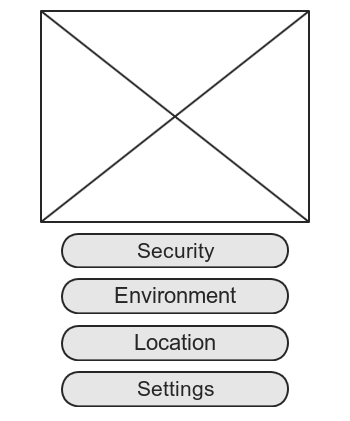
\includegraphics[scale=0.5]{mock_home}
    \caption[Wireframe of the home screen]
            {Wireframe of the home screen}
    \label{fig:wireframe-home}
\end{figure}

\begin{figure}[H]
    \centering
    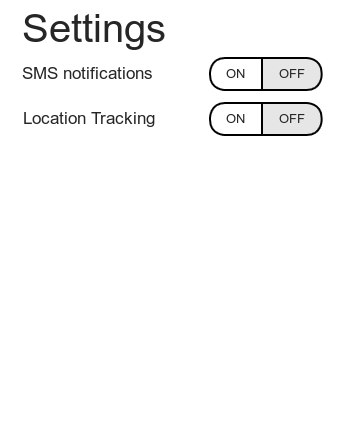
\includegraphics[scale=0.5]{mock_settings}
    \caption[Wireframe of the settings screen]
            {Wireframe of the settings screen}
    \label{fig:wireframe-settings}
\end{figure}

Various portions of the security system can be controlled through the wireframe
in Figure~\ref{fig:wireframe-security}. The entire system can be armed and
disarmed, locks on doors activated and deactivated, and the status of the
windows can be reported. Pressing on the button for window status will bring up
another more detailed screen that lists individual windows and reports their
status, closed or open. Door locks, if it is supported can be locked or
unlocked from this screen if the lock supports it.


\begin{figure}[H]
    \centering
    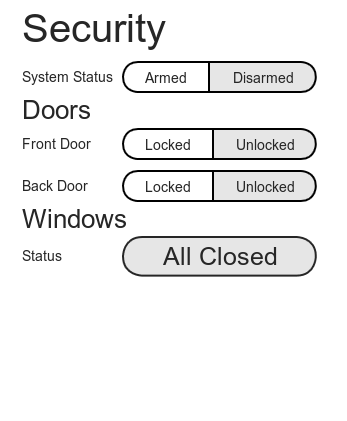
\includegraphics[scale=0.5]{mock_security}
    \caption[Wireframe of the security screen]
            {Wireframe of the security screen}
    \label{fig:wireframe-security}
\end{figure}

Environmental details are controlled in Figure~\ref{fig:wireframe-environment}. The
temperature of the house can be monitored and set. Pressing on the button
labeled ``HISTORY'' will bring up a graph of the household temperature over a
period of time. This screen can also display images from cameras at the doors
to allow for the user to check who is at the door before unlocking it.
Details from more specific portions of the enviroment can be displayed here as
well. For example, the status of the stove and oven in the kitchen. It is also
possible to report the internal temperature of the oven to ensure that it is
not overheating.

\begin{figure}[H]
    \centering
    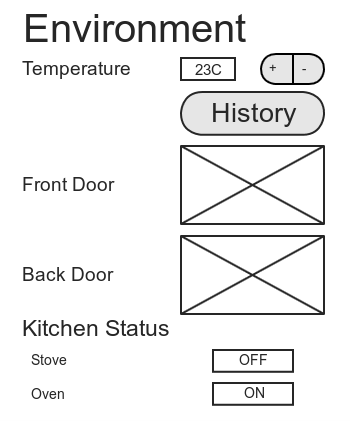
\includegraphics[scale=0.5]{mock_environment}
    \caption[Wireframe of the environment screen]
            {Wireframe of the environment screen}
    \label{fig:wireframe-environment}
\end{figure}

Family member locations -- at least those with smartphones and this
application -- are displayed in Figure~\ref{fig:wireframe-locations}. Each family
member will have a pin on the map to show their location using their device's
GPS capabilities. Clicking on a name will move the map to the present location
of that person. It will also display in text where the family member presently
is located.

\begin{figure}[H]
    \centering
    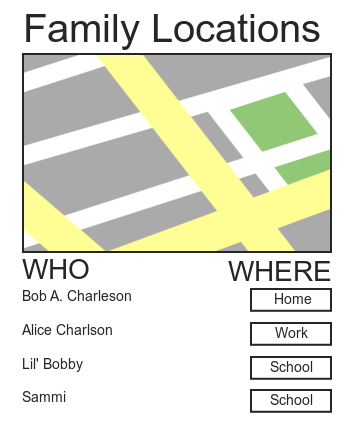
\includegraphics[scale=0.5]{mock_locations}
    \caption[Wireframe of the locations screen]
            {Wireframe of the locations screen}
    \label{fig:wireframe-locations}
\end{figure}



\section{Near-field Communication Keypad}
A keypad located near the main entrances to the house provides a physical
interface to setting the security system and other states. Two methods are
provided for arming and disarming. The first is near-field communication if the
user's smartphone supports it. Authentication is done with a simple tap of the
device to the keypad and then the user can set the state of the system. The
other authentication method is for the user to input their unique keycode. The
intention of this keypad is a fallback method in case the user does not have a
smart phone or if they have mis-placed it.

\section{Web Server}
\label{sec:web-server}
% TODO :: move this into the Functional Reqs?
A web server serves two purposes. It provides an interface between the mobile
application described in Section~\ref{sec:mobile-app} and the system
controller. Data can be accessed remotely through API requests and the state of
the system can be modified by sending requests to it. The other purpose is to
maintain a log of all the events for trend analysis and household history. The
server should be located at a remote location for data security.  A graphical
frontend implemented on the server will also allow for remote monitoring when
the user does not have their phone on their person. 


\end{document}
